%!TEX root =  ../main.tex

\subsection{$r, \theta$}
Apart from arbitrary roads running north-south and east-west, no one would ever walk solely
in horizontal and vertical lines.  When you want to fly your plane somewhere, you turn the
nose towards where you want to go, and walked the shortest path.  For example, you might
know that your friend is 3m east of you and 4m north, but you would never walk the 7m such 
ludacrous path takes.  What is the shortest path ($r$)?  What angle would you turn ($\theta$)?

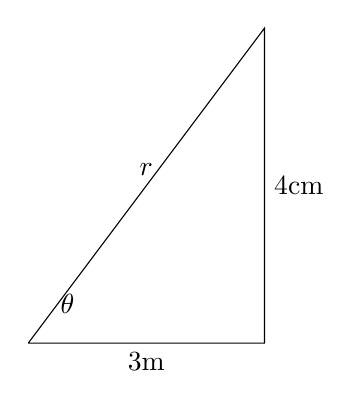
\begin{tikzpicture}
	\draw (0,0) -- (3,0) -- (3,4) -- (0,0);
	\draw (1.5,0) node[anchor=north] {3m};
	\draw (3,2) node[anchor=west] {4cm};
	\draw (1.5,2) node[anchor=south] {$r$};
	\draw (0.5,0.5) node {$\theta$};
\end{tikzpicture}

Well, by this point in this class, you are undoubtedly very used to using the Pythagorean Theorem
to find hypotenuses, and inverse tangent to calculate angle.  While you should certainly be able to
calculate $r=5$, a calculator or table is required to know when tangent is $1.\overline{3}$, 
approximately 0.927 radians.

On the other hand, suppose you knew something was 6 miles away, at an angle of $\frac{2}{3}\tau$.
How would you determine how far east-west and north-south it is?  Just as we learned with vectors,
we can use sine and cosine to calculate these values.  $\sin(\frac{2}{3}\tau)=\frac{y}{6}$ and 
$\cos(\frac{2}{3}\tau)=\frac{x}{6}$.  Solving for $x$ and $y$, we see the coordinates of the
destination are $(-3,-3\sqrt{3})$.

So in generally, we can derive four formulae:
\begin{itemize}
\item $r^2=x^2+y^2$
\item $\tan\theta=\frac{y}{x}$*
\item $x=r\cdot\cos\theta$
\item $y=r\cdot\sin\theta$
\end{itemize}
The tangent equation doesn't work everywhere: what are the limitations on how we can use it?

\subsection{Properties}
Working with $r$ and $\theta$ to the exclusion of $x$ and $y$ yields a different way of looking
at the coordinate plane, called \emph{polar coordinates}.  Locations are still labeled via ordered
pairs, but of the form $(r,\theta)$.  Polar graph paper looks like this:

  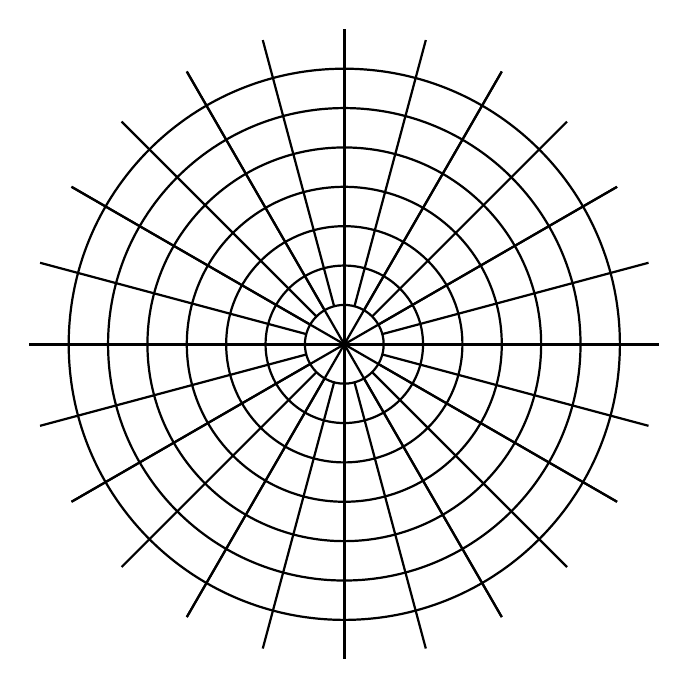
\begin{tikzpicture}[scale=0.5]
    %Circles 
    \foreach \r in {1, 2,...,7}
      \draw[thick] (0,0) circle (\r);    
     %half radii 
    %\foreach \r in {0.5, 1.5,...,7}
      %\draw[thin] (0,0) circle (\r);
    %1° Rays
    %\foreach \a in {0, 1,...,359}
      %\draw[-] (\a:7.7) -- (\a:8);
    %5° Rays
    %\foreach \a in {0, 5,...,359}
      %\draw[-] (\a:7.5) -- (\a:8);      
    %15° Rays
    \foreach \a in {0, 15,...,359}
      \draw[thick] (\a:1) -- (\a:8); 
    %30° Rays
    \foreach \a in {0, 30,...,359}
      \draw[thick] (0, 0) -- (\a:8);
    %Radius labels (background filled white)
    %\foreach \r in {1, 2,...,7}
      %\draw (\r,0) node[inner sep=1pt,below=3pt,rectangle,fill=white] {$\r$};
    %Main rays
    \foreach \a in {0, 90,...,359}
      \draw[very thick] (0, 0) -- (\a:8);
\end{tikzpicture}

\subsection{Negative Radii}
The ``spokes'' are every $\frac{\tau}{24}$, and the circles are every unit.  You might begin by turning
the angle first, and then ``walking out'' the radius.  On the polar graph, try locating $(3,\frac{\tau}{4})$.
It shouldn't be too complicated to see this is the same as the rectangular coordinate (0,3).  Angles
greater than $\tau$ are not difficult to reduce to simpler terms, but what about negative radii?  
Where would $(-3,\frac{3}{4}\tau)$ take you?  We might imagine a person standing at the
pole (the origin on a polar graph), he or she would begin facing to the right, and then turning 
counter-clockwise.  $\frac{3}{4}\tau$ is straight down, so our person's back is to the ``north''.  A
negative radii can be thought of as walking \emph{backwards}, so $(3,\frac{\tau}{4})$ and
$(-3,\frac{3}{4}\tau)$ take you to the same place!


\subsection{Polar Equations}
Just as Cartesian (or rectangular) equations as $y$ equals something in terms of $x$, so
too polar equations are written as $r$ equals something in terms of $\theta$.  Press the `mode'
button on your calculator, and you can see that there is an option called `POL', short for POLAR.
Accept that option and see what the `y=' button has become!  What has the X button become?

The exercise or problems will walk you through many different types of $r=$ equations, and they
can all be demonstrated in your calculator.  However, just as you have to know how to graph
$x=n$ even though it is not a function in rectangular, so too you should take a moment and reason
through how to graph $\theta=\frac{1}{5}\tau$ and similar equations. 

When we attempt plot points to determine the make-up of $x=3$, we see that $y$ can be anything.
In other words, (3,0); (3,1); (3,2); (3,-2); (3,-10), etc. are all on the graph.  When we take this principle
over to graphing $\theta=\frac{5}{6}$, we recognize that any radius is possible, including negatives.
~\vfill
